\documentclass[10pt,a4paper]{article}
\usepackage[margin=17mm,top=15mm,bottom=16mm]{geometry}
\usepackage{amsmath,amssymb,bm}
\usepackage{graphicx}
\usepackage{booktabs}
\usepackage{newtxtext,newtxmath}
\usepackage{caption}
\usepackage{enumitem}
\usepackage[hidelinks]{hyperref}
\captionsetup{font=small,labelfont=bf,labelsep=quad,skip=3pt,justification=centering}
\setlist[itemize]{leftmargin=1.1em,itemsep=0pt,topsep=2pt,parsep=0pt}
\setlength{\columnsep}{6mm}
\setlength{\columnwidth}{\dimexpr(\textwidth-\columnsep)/2\relax}
\setlength{\parindent}{1em}
\renewcommand{\baselinestretch}{0.98}
\setlength{\emergencystretch}{2em}
\pagestyle{empty}

\newcommand{\ket}[1]{\lvert #1\rangle}
\newcommand{\bra}[1]{\langle #1\rvert}
\newcommand{\braket}[2]{\langle #1\vert #2\rangle}
\newcommand{\bramat}[3]{\langle #1\vert #2\vert #3\rangle}

\begin{document}

\twocolumn[{%
\begin{center}
{\large\bfseries Matrix-Free Deflation for Frozen-Subspace Neural Excited-State\\[1pt] Variational Monte Carlo}\\[3pt]
{\normalsize (Japanese translation of the title to be inserted here)}\\[6pt]
\begin{tabular}{ll}
Supervising professor: & Prof.\ [name]\\
Student ID number: & [number]\hspace{4mm}Name: [name]
\end{tabular}
\end{center}
\vspace{-1mm}
}]

\section{Introduction}

Electronic excited states are central to spectroscopy, photochemistry and materials modelling, yet they remain the weak point of variational Monte Carlo (VMC). Full configuration interaction (FCI) is exact within a one-electron basis\ \textsuperscript{1)} but scales factorially, so practical calculations must rely on compact, explicitly correlated wave functions. Neural-network quantum states (NQS)\ \textsuperscript{2)} supply such wave functions: amplitudes and local energies are evaluated pointwise on configurations drawn by Markov-chain Monte Carlo (MCMC)\ \textsuperscript{11)}, the Hamiltonian acts through its sparse connection graph, and the parameters are optimised by stochastic reconfiguration (natural gradient)\ \textsuperscript{3,4)}. Neither the state nor the Hamiltonian is ever stored as a $2^N$-dimensional object, which is why NQS-VMC can reach Hilbert spaces far beyond exact diagonalisation.

Excited states break this scheme, because a Rayleigh quotient is minimised by the ground state. Standard remedies are orthogonalisation against lower states, penalty or variance-based functionals\ \textsuperscript{5,6)}, and symmetry restriction\ \textsuperscript{7)}. Natural excited-state VMC (NES-VMC)\ \textsuperscript{8)} instead optimises $K$ states jointly through a determinant on a $K$-fold replicated configuration space, so that $K$ eigenpairs are obtained from one MCMC run.

The price of joint optimisation is that all $K$ states are coupled: every additional state enlarges the replicated walker, the local-energy matrix, the parameter set and the stochastic-reconfiguration system, and it perturbs states that are already converged. In our H$_2$/6-31G calculations the two members of a spin-degenerate pair are typically the ones left behind, by up to 3.8~mHa, because they are nearly linearly dependent inside the determinant.

The alternative, deflation, is the standard tool of iterative eigensolvers\ \textsuperscript{9)} and of embedded correlation methods\ \textsuperscript{10)}: once a set of eigenpairs is known, new ones are computed in the complementary invariant subspace, and the known ones are never revisited. Applying it to neural quantum states is not a matter of transcription. A neural state exists only as a function, not as a vector; the projection coefficients are full-space inner products whose direct evaluation would reintroduce the exponential cost; the Hamiltonian is available only through its local connections; and sampling, estimator and gradient must remain mutually consistent after the projection.

This work recycles instead of re-optimising. Once a small set of low-lying states is converged, they are \emph{frozen} and used as a fixed basis; only a few new states are optimised, and only in the orthogonal complement of that basis. The key difficulty is that a neural state is a function, not a vector: the projection requires Hilbert-space inner products between frozen and active columns, and a naive evaluation would reintroduce the exponential cost. We show that these coefficients can be obtained from Monte Carlo estimates of Gram matrices sampled on an auxiliary distribution, with the unknown normalisation cancelling exactly, and that the projection is then enforced automatically by the determinant -- no $2^N$ vector, no dense Hamiltonian and no explicit projector is ever formed. Section~2 develops the formulation, Section~3 reports H$_2$/6-31G and LiH/STO-3G results, and Sections~4--6 discuss limitations, conclusions and the research plan.

\section{Method}

\begin{figure}[t]
\centering
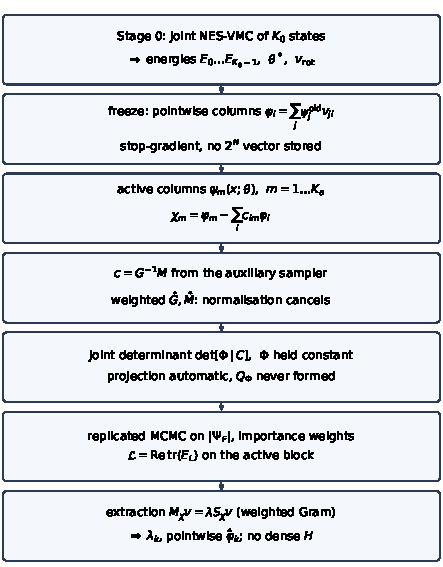
\includegraphics[width=80mm]{figures/fig1_framework.pdf}
\caption{Matrix-free frozen-subspace expansion. A converged $K_0$-state solution is split into frozen columns (pointwise functions, stop-gradient) and a small number of fresh active columns; the projection coefficients come from an auxiliary sampler; the joint determinant enforces the projection implicitly; energies are extracted from a weighted generalised eigenproblem. No $2^N$ vector and no dense Hamiltonian appear at any stage.}
\label{fig:flow}
\end{figure}

The overall construction is summarised in Fig.~1. The pipeline has five ingredients: (i) a converged joint solution that defines the frozen basis, (ii) pointwise frozen columns obtained by a small rotation of the old networks, (iii) Monte Carlo Gram matrices that fix the projection coefficients, (iv) a joint determinant in which the frozen block is constant, and (v) a weighted generalised eigenproblem that yields the physical energies and states.

\subsection{NES-VMC in matrix-free form}

In NES-VMC the $K$ single-state wave functions $\psi_0,\dots,\psi_{K-1}$ are combined into a determinant on replicated configurations $\mathbf{x}=(\mathbf{x}_1,\dots,\mathbf{x}_K)$,
\begin{equation}
\Psi_\theta(\mathbf{x})=\det\bigl[\psi_j(\mathbf{x}_i)\bigr]_{i,j=0}^{K-1},
\end{equation}
and for each replica the amplitudes $A_{ij}=\psi_j(\mathbf{x}_i)$, the Hamiltonian action $Z_{ij}=(H\psi_j)(\mathbf{x}_i)$ and the local-energy matrix $E_L=A^{-1}Z$ define the loss
\begin{equation}
\mathcal{L}(\theta)=\operatorname{Re}\operatorname{tr}\langle E_L\rangle .
\end{equation}
The physical states and energies follow from the subspace Ritz problem, with $S_{ij}=\braket{\psi_i}{\psi_j}$ and $M_{ij}=\bramat{\psi_i}{H}{\psi_j}$,
\begin{equation}
Mv=\lambda Sv,
\end{equation}
estimated on the sampled configurations. No matrix element is ever evaluated in the full Hilbert space; $H\psi_j$ is obtained from the local connections of $\mathbf{x}_i$.

Two cost statements follow directly from Eqs.~(1)--(3). The replicated walker is $K$ configurations of $N$ spin orbitals, so the sampling cost is linear in $K$ and linear in the number of local connections per configuration; the local-energy matrix is $K\times K$, and its inversion supplies both the loss and the gradient. The problematic term is the parameter set: all $K$ networks are optimised simultaneously, so the stochastic-reconfiguration system has dimension $K$ times the single-network parameter count, and the number of variational parameters -- not the Hilbert-space dimension -- is what limits the practical value of $K$.

\subsection{Frozen basis and projection coefficients}

Let $\psi_j^{\rm old}(\cdot;\theta^*)$, $j=0,\dots,J-1$, be a converged joint solution and $v_{\rm rot}$ the rotation that diagonalises its Ritz problem. We retain $r\le J$ of its columns and represent each frozen state pointwise,
\begin{equation}
\varphi_i(x)=\sum_{j=0}^{J-1}\psi_j^{\rm old}(x;\theta^*)\,v_{ji},
\qquad i=0,\dots,r-1,
\end{equation}
so that $\varphi_i$ is a plain function of $x$ with no stored vector and no gradient. New active columns $\psi_m(x;\theta)$, $m=1,\dots,K_a$, enter only through their components orthogonal to the frozen span,
\begin{equation}
\chi_m=\psi_m-\sum_{i=0}^{r-1}c_{im}\varphi_i,
\end{equation}
where the coefficient matrix obeys
\begin{equation}
c=G^{-1}M,
\end{equation}
with $G_{ij}=\braket{\varphi_i}{\varphi_j}$ and $M_{im}=\braket{\varphi_i}{\psi_m}$ the Gram matrices of the two sets.

The inner products in $G$ and $M$ are the only genuinely non-local objects in the construction. They are estimated by importance sampling on an auxiliary distribution
\begin{equation}
q(y)\propto\sum_{i=0}^{r-1}\lvert\varphi_i(y)\rvert^2
+\varepsilon\sum_{m=1}^{K_a}\lvert\psi_m(y)\rvert^2 ,
\end{equation}
whose purpose is to cover both the frozen and the active support, since the active states are still far from converged at the beginning of the run. Writing $Z_q=\sum_y q(y)$ for the unknown normalisation, every Gram block estimated on the same sample carries the same factor, $\hat G=G/Z_q$, $\hat M=M/Z_q$, hence
\begin{equation}
\hat G^{-1}\hat M=\bigl(G/Z_q\bigr)^{-1}\bigl(M/Z_q\bigr)=G^{-1}M .
\end{equation}
The normalisation cancels identically, so neither a wave-function norm nor a full-space overlap has to be computed. In practice $G$ is regularised by a small diagonal shift and by a truncated pseudo-inverse, and $c$ is only meaningful for columns that remain linearly independent of the frozen set.

\subsection{Determinant with a frozen block}

The projected columns are placed next to the frozen ones, $\Phi=[\varphi_0,\dots,\varphi_{r-1}]$ and $C=[\chi_1,\dots,\chi_{K_a}]$, in a single determinant,
\begin{equation}
\Psi_F=\det[\,\Phi\,|\,C\,].
\end{equation}
Because $\chi_m$ already contains the subtracted frozen part, the determinant is invariant under adding any linear combination of the frozen columns to an active column, i.e.\ $\det[\Phi\,|\,C]=\det[\Phi\,|\,Q_\Phi C]$ with $Q_\Phi$ the orthogonal projector onto the complement of $\operatorname{span}\Phi$. The projection is therefore enforced \emph{automatically} by the antisymmetriser, and differentiating the determinant yields the projected tangent-space gradient without ever constructing $Q_\Phi$. In the implementation the frozen block $[\Phi]$ is a constant: its amplitudes are evaluated with the frozen parameters under a stop-gradient, and only $\theta$ and the coefficient matrix $C$ are differentiated. Sampling is done on the replicated distribution $|\Psi_F|^2$ with importance weights, and the loss of Eq.~(2) is evaluated on the active block only.

\subsection{Extraction and the correct energy estimator}

Physical energies are extracted from a generalised eigenvalue problem built from the active columns, with $(S_\chi)_{mn}=\braket{\chi_m}{\chi_n}$ and $(M_\chi)_{mn}=\bramat{\chi_m}{H}{\chi_n}$,
\begin{equation}
M_\chi v=\lambda S_\chi v,
\end{equation}
estimated on consistently weighted samples so that the same normalisation cancellation applies. The estimator matters: eigenvalues of the sample-averaged local-energy matrix, $\operatorname{eig}\langle E_L\rangle$, reproduce only $\operatorname{tr}\mathcal{L}$ and are \emph{not} the subspace eigenvalues for $K\ge2$; in our H$_2$ run they undershoot the extraction values by more than an order of magnitude in accuracy (0.098 vs.\ 0.009~mHa for the same run). Equation~(11) is the quantity to report.

\subsection{Training algorithm}

One expansion cycle is organised as follows.
\begin{enumerate}[leftmargin=1.4em,itemsep=0pt,topsep=2pt,parsep=0pt]
\item Load a converged $J$-state solution $(\theta^*,v_{\rm rot})$ and diagonalise its Ritz problem; select the $r\le J$ columns to freeze.
\item Build the frozen columns as pointwise functions, Eq.~(4), and record their scales; the old parameters are kept but never updated.
\item Draw auxiliary samples from $q$, Eq.~(7), and accumulate $\hat G$ and $\hat M$; solve for $c$ with a diagonal shift and a truncated pseudo-inverse.
\item Draw main samples from the replicated distribution $|\Psi_F|^2$, evaluate $\Psi_F=\det[\Phi|C]$, the local-energy matrix and the loss of Eq.~(2) on the active block.
\item Update only $\theta$ and $C$ by stochastic reconfiguration, rescaling the columns with exponential moving averages; the frozen block enters as a constant reference.
\item Every few steps, solve the weighted eigenproblem of Eq.~(10) and monitor $\lambda_k$ together with the diagnostics of Section~3.3.
\item At the end, extract $\lambda_k$ and the corresponding pointwise recipes; no dense object is written to disk.
\end{enumerate}
The auxiliary sampler is what makes the scheme practical: it converts full-space inner products into ordinary Monte Carlo averages, at the price of one extra sampling stage whose distribution has to cover both the frozen and the active support.

Two numerical safeguards are worth mentioning. First, the column scales of the active networks drift during training, and the projection coefficients must be transformed together with them; otherwise the frozen subtraction becomes inconsistent and the determinant loses rank. We therefore keep exponential moving averages of the scales and apply the corresponding similarity transformation to $c$. Second, sampling the replicated distribution $|\Psi_F|^2$ with frozen columns gives zero-variance amplitudes for the frozen block when only active columns change, which would freeze the estimator; the importance-weighted loss removes this degeneracy by reweighting each replica with the ratio of the current to the sampling distribution.

\subsection{Error budget}

The retrieved level can be written as the projected Rayleigh quotient plus two corrections,
\begin{equation}
\lambda_k=\frac{\bramat{\chi_k}{H}{\chi_k}}{\braket{\chi_k}{\chi_k}}
=\lambda_k^{\rm proj}+\Delta_k^{\rm proj}+\Delta_k^{\rm stat},
\end{equation}
where the projection bias is controlled by the residual of the frozen manifold and the statistical term by the effective sample size,
\begin{equation}
\lvert\Delta_k^{\rm proj}\rvert
\lesssim
\frac{\lVert(1-P)H P\chi_k\rVert}{\lVert\chi_k\rVert}
+\mathcal{O}\bigl(\eta_{\rm fr}^2\bigr),
\end{equation}
and the statistical term is set by the effective sample size,
\begin{equation}
\Delta_k^{\rm stat}\sim\sqrt{\operatorname{Var}\bigl[\hat\lambda_k\bigr]/N_{\rm eff}} .
\end{equation}
with $P$ the projector onto $\operatorname{span}\Phi$ and $\eta_{\rm fr}$ the frozen residual. The two corrections are what make the diagnostics actionable: $\Delta^{\rm proj}$ is invisible in the loss, vanishes when the frozen states are exact eigenstates, and is the term that an oracle diagonalisation of $QHQ$ isolates. Because the two terms cannot be measured separately in a single run, we use the disagreement between the per-step monitor and the final extraction (Table~3) as a proxy for their sum: it is 0.03--0.17~mHa for the small blocks and exceeds 1~mHa once six active columns are used.

\section{Results}

\subsection{H$_2$/6-31G}

The first benchmark is H$_2$ in the 6-31G basis, CAS(2e,4o), i.e.\ eight spin orbitals and a 16-dimensional FCI space; the FCI ground state is $E_0=-1.05434745$~Ha. All training uses $16\times200$ MCMC chains with 20 sweeps, natural-gradient steps with $\mathrm{lr}=0.1$ and diagonal shift $0.1$, and an auxiliary sampler with 1024 chains and $\epsilon=0.25$. Dense Hamiltonians and FCI vectors are used for diagnostics only.

Table~1 and Fig.~2 summarise the outcome. Starting from a frozen four-state solution, adding four active states recovers $E_4$--$E_7$ with a maximum error of 0.009~mHa in 500 steps and 425~s, i.e.\ an order of magnitude better than a direct $K=6$ optimisation that needed about 26~min for 1000 steps and still left $E_1$ and $E_4$ at 3.8~mHa. Adding only two active states is cheaper but leaves the second new level 0.8~mHa off, and adding six active states degrades the two highest levels (1.05 and 1.38~mHa), which indicates that the useful active-block size is set by conditioning rather than by cost alone. The same trend is visible in Fig.~2(b): the $K_a=4$ block is uniformly accurate, while larger or smaller blocks fail for particular levels.

Expanding from a larger frozen manifold behaves differently. With $K_0=6$ frozen, two active states recover $E_6$ and $E_7$ to 0.18 and 0.03~mHa, and four active states recover $E_6$--$E_9$ to 0.53, 0.03, 0.07 and 0.34~mHa, again with the lowest of the new levels being the hardest. Six active states starting from $K_0=6$ are markedly worse (0.23--0.47~mHa for four of the six levels) even though the frozen manifold is larger: the active determinant is then twelve-dimensional and the sampled Gram matrices lose conditioning. This is consistent with the observation above and defines the practical operating point $K_a\le4$ for the present network family and sampler settings.

A further point concerns the direct $K=6$ run: it is not simply inaccurate, it is seed-dependent. With one initialisation it reaches 0.31~mHa in 500 steps, with another it stalls at 3.8~mHa after 1000 steps, and in both cases the stalled levels are the two members of the spin-degenerate pair. Frozen-subspace expansion removes this variance for the protected states by construction, because their parameters are never updated; the remaining variance is confined to the new columns.

\begin{table}[t]
\centering
\caption{Energies of H$_2$/6-31G relative to FCI (mHa); ``init.~a/b'' marks two different seeds. Direct runs are judged by the per-step Ritz monitor, expansion runs by the weighted Gram estimator of Eq.~(10).}
\label{tab:h2}
\small
\setlength{\tabcolsep}{3.2pt}
\begin{tabular}{@{}llcccc@{}}
\toprule
\textbf{Run} & \textbf{setting} & \textbf{levels} & \textbf{steps} & \textbf{time} & \textbf{error}\\
\midrule
direct & K=4, init.~a & 0--3 & 300 & 3 min & 0.18\\
direct & K=6, init.~a & 0--5 & 1000 & 26 min & 3.81\\
direct & K=6, init.~b & 0--5 & 500 & -- & 0.31\\
\midrule
frozen & K0=4, Ka=2 & 4--5 & 500 & 185 s & 0.81\\
frozen & K0=4, Ka=4 & 4--7 & 500 & 425 s & 0.009\\
frozen & K0=4, Ka=6 & 4--9 & 500 & 964 s & 1.38\\
\bottomrule
\end{tabular}
\end{table}

\begin{figure}[t]
\centering
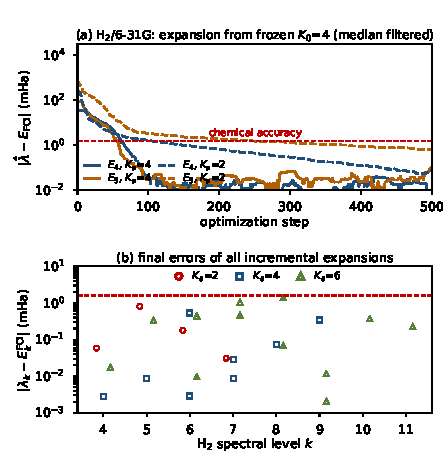
\includegraphics[width=80mm]{figures/fig2_convergence.pdf}
\caption{Matrix-free expansion for H$_2$/6-31G. (a) Running error of the Ritz monitor during the optimisation for a frozen $K_0=4$ solution with $K_a=4$ (solid) and $K_a=2$ (dashed); curves are median filtered to suppress estimator noise. (b) Final errors of all incremental runs, evaluated with the weighted Gram estimator. $K_a=4$ is uniformly accurate; small or large active blocks leave individual levels behind.}
\label{fig:h2}
\end{figure}

\subsection{LiH/STO-3G}

The second benchmark is LiH in STO-3G, CAS(2e,4o), again eight spin orbitals (FCI dimension 36). Here the spectrum is dominated by two spin-degenerate pairs at 167.4 and 188.3~mHa above the ground state. The direct $K=4$ solution reproduces the ground state and one member of each pair but ranks a spurious second state 2.6~mHa too high (Fig.~3); freezing its columns $(0,1,3)$ and optimising three new columns recovers the partners $E_2$, $E_4$ and the next level $E_5$ to 0.0008, 0.0061 and 0.0003~mHa, in 500 steps and 282~s. The full $K=6$ optimisation needs 15~min for the same number of steps and reaches 0.067~mHa (Table~2). The frozen columns were never touched during the expansion, so the already converged ground state stayed at 0.002~mHa.

\begin{table}[t]
\centering
\caption{LiH/STO-3G, CAS(2e,4o), eight spin orbitals. Errors in mHa relative to FCI; wall-clock times from the run logs of one workstation.}
\label{tab:lih}
\small
\setlength{\tabcolsep}{3.5pt}
\begin{tabular}{@{}llcccc@{}}
\toprule
\textbf{Run} & \textbf{setting} & \textbf{levels} & \textbf{steps} & \textbf{time} & \textbf{error}\\
\midrule
direct & K=4 & 0--3 & 500 & 9 min & 2.65\\
direct & K=5 & 0--4 & 500 & 9 min & 0.024\\
direct & K=6 & 0--5 & 500 & 15 min & 0.067\\
frozen & K0=4, Ka=3 & 2,4,5 & 500 & 282 s & 0.006\\
\bottomrule
\end{tabular}
\end{table}

\begin{figure}[t]
\centering
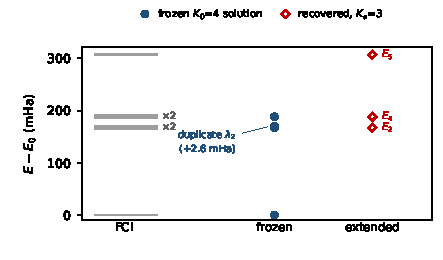
\includegraphics[width=80mm]{figures/fig3_lih.pdf}
\caption{LiH/STO-3G level diagram. Grey bars: FCI multiplets (spin-degenerate partners are drawn with a small vertical offset). Filled circles: the four states of the direct $K_0=4$ solution; one of them is a duplicate $2.6$~mHa above the pair. Diamonds: states recovered by three active columns, which restore both degenerate partners and the next level.}
\label{fig:lih}
\end{figure}

\subsection{Diagnostics}

Four quantities are monitored during the run: the fraction of valid walkers ($1.00$ throughout), the effective sample size of the main sampler (typically $0.75$--$0.80$ of $3200$ walkers), the effective sample size of the auxiliary sampler ($\approx35\%$ of 1024 chains, the limiting cost of the method), and the condition number of the sampled Gram matrix ($\kappa\approx3$--$6$ for $K_a\le4$, growing quickly beyond). A growing $\kappa$ together with a stalled loss indicates genuine optimisation failure, whereas a stalled monitor with a healthy $\kappa$ is usually the estimator bias discussed in Section~2.4; the two must be separated before any conclusion about the frozen-subspace bias is drawn.

\subsection{Internal consistency of the implementation}

Table~3 collects the same quantities for all six H$_2$ expansions. The clipping counter counts the steps at which the stochastic-reconfiguration update had to be clipped: it is zero for the four-state and six-state parents with $K_a\le2$, three for $K_0=6$ with $K_a=4$, and thirty for $K_a=6$, which is the signature of an ill-conditioned active block rather than of a bad sampler. The final loss follows the same pattern. The last two columns compare the per-step Ritz monitor with the extraction of Eq.~(10); the two are computed from different sample sets and different matrices, so their agreement is an internal consistency check of the whole chain -- frozen columns, coefficients, weights and normalisation cancellation. For $K_a\le4$ the two agree within 0.34~mHa, which is the resolution of the monitor at that statistics; the disagreement above 1~mHa for $K_a=6$ is the same conditioning problem, and it is the reason why we report the extraction rather than the monitor as the final number.

\begin{table}[t]
\centering
\caption{H$_2$/6-31G expansion runs: clipped updates, final loss, and the deviation between the per-step monitor and the extraction (mHa).}
\label{tab:diag}
\small
\setlength{\tabcolsep}{3.2pt}
\begin{tabular}{@{}lccccc@{}}
\toprule
\textbf{Run} & \textbf{Ka} & \textbf{clip} & \textbf{loss} & \textbf{mon.--ext.} & \textbf{time}\\
\midrule
K0=4 & 2 & 0 & −0.042 & 0.17 & 185 s\\
K0=4 & 4 & 0 & −0.024 & 0.09 & 425 s\\
K0=4 & 6 & 0 & 0.468 & 1.27 & 964 s\\
K0=6 & 2 & 0 & 0.019 & 0.03 & 233 s\\
K0=6 & 4 & 3 & 0.510 & 0.34 & 539 s\\
K0=6 & 6 & 30 & 1.510 & 1.51 & 1302 s\\
\bottomrule
\end{tabular}
\end{table}

\subsection{Implementation and reproducibility}

The implementation follows the matrix-free contract literally. Amplitudes are complex phase/amplitude networks evaluated with JAX under NetKet, and the Hamiltonian is applied through its connection list, so neither the state nor $H$ is ever assembled; a dense Hamiltonian and the FCI eigenvectors are computed separately, in a diagnostic script, and are used only to evaluate errors and to validate each matrix-free quantity against its exact counterpart on the 16- and 36-dimensional spaces. Each run writes three artefacts: a log with per-step diagnostics, a history file with the Ritz values and losses, and an extraction file with $\lambda_k$, the rotation $v_{\rm rot}$, the coefficient matrix $c$, the column scales and the elapsed time. The same initial seed (11) and hyperparameters are used throughout, so the differences in Table~1--3 reflect the block sizes and not the random stream. All timings quoted above are wall-clock times of the same single workstation, measured from the logs, and include the auxiliary sampling stage.

This separation between production and diagnostic code is what makes the claims checkable: every quantity that the method uses in production is recomputed exactly for the small benchmarks, so an error in the Gram estimation, in the normalisation cancellation or in the projection would appear as a disagreement in Table~3 rather than as a slow drift of an energy.

\section{Discussion and limitations}

The construction is dimension-free: the training loop touches only pointwise amplitudes, local connections and small $K_a\times K_a$ matrices, so its cost grows with the number of active states, not with the Hilbert-space size. Memory follows the same rule -- the state is a set of network parameters, and the only matrices stored are the $r\times r$, $r\times K_a$ and $K_a\times K_a$ Gram blocks and the coefficient matrix. For the present benchmarks this is a few megabytes, independent of the 16- or 36-dimensional FCI space; the point is that the same statement remains true when the active space grows to the point where a dense object would not fit in memory at all.

Three limitations remain. First, the frozen states are approximate eigenstates, so the projected problem carries an intrinsic bias of the order of the frozen residual; an oracle diagonalisation of $QHQ$ separates this bias from optimisation error and shows that the current 0.009~mHa level is dominated by the expressivity of the active networks rather than by projection. This also means that the method cannot be made arbitrarily accurate by adding states: a poorly converged frozen manifold limits what the complement can contain. Second, the auxiliary sampler is the bottleneck. Its effective sample size, not the gradient step, sets the wall-clock cost, and because the distribution has to cover both the frozen and the active support its efficiency degrades as the active columns grow. Third, the active block is fragile for $K_a\ge6$: near-linear dependence inflates the condition number, the pseudo-inverse truncates legitimate directions, and individual levels are left behind (1.05 and 1.38~mHa in Table~1). A preconditioner, or an adaptive rule for $K_a$, is needed for larger expansions.

Compared with penalty and variance-based excited-state functionals, the approach does not require tuning a penalty weight, and it yields several states per run with a single hyperparameter set. Compared with a full $K$-state optimisation, it trades a small amount of bookkeeping -- one auxiliary sampler and one Gram solve -- for the guarantee that converged states are not revisited. The price is that the frozen manifold is fixed: improving a frozen state requires a new expansion cycle from a better parent calculation.

\section{Conclusion}

Frozen-subspace recycling turns excited-state NES-VMC from a joint re-optimisation into an incremental one. Frozen states are reused as pointwise functions, projection coefficients come from Monte Carlo Gram matrices with exact normalisation cancellation, the determinant enforces the projection implicitly, and the weighted Gram eigenvalue problem supplies the physical energies. On H$_2$/6-31G four frozen states plus four active states reach $0.009$~mHa for $E_4$--$E_7$ in 425~s, and on LiH/STO-3G three active states recover the degenerate partners missed by the direct calculation at $0.006$~mHa. No $2^N$ vector, dense Hamiltonian or explicit projector is constructed at any stage.

Two aspects seem to me the essential outcome of this period. The first is conceptual: deflation, a purely vector-space operation in conventional eigensolvers, survives the transition to neural quantum states once the inner products are recognised as Monte Carlo expectations on an auxiliary distribution and the unknown normalisations are allowed to cancel. The second is practical: the incremental strategy is not merely cheaper than a joint optimisation, it is also more stable, because the states that a determinant of nearly dependent columns cannot hold are protected by construction once they are frozen. Both statements are supported here by controlled benchmarks where the exact answer is known; the open question is whether they survive at the system sizes where the matrix-free formulation is not just convenient but necessary.

\section{Research plan after enrolment}

The next step is to move from benchmark molecules to a systematically improvable excited-state workflow. (i) Extend the benchmarks to LiH/cc-pVDZ, H$_2$O and N$_2$ in active spaces of 12--20 spin orbitals, where the exponential cost of any dense object becomes prohibitive and the matrix-free property can be demonstrated rather than asserted; the first target is LiH with a 12-orbital active space, for which a direct $K=6$ optimisation already exceeds the memory of a single workstation once a dense Hamiltonian is formed. (ii) Replace single-run estimates by statistically controlled ones: variance-based error bars, reblocking and multi-seed averages for both energies and overlaps, so that every reported number carries an uncertainty. (iii) Improve the conditioning of the active block with natural-orbital rotations, a truncated pseudo-inverse with an explicit threshold, and an adaptive rule for the number of active states -- the $K_a\ge6$ degradation in Table~1 is the concrete problem to solve. (iv) Accelerate the auxiliary sampler, which currently dominates the cost, by reweighting from the main sampler and by batching on GPUs. (v) Combine the frozen basis with spin and spatial symmetry labels, so that degenerate manifolds are frozen as multiplets rather than as individual columns, and interface the extraction with a conventional quantum-chemistry code for comparison with EOM-CCSD. The goal is a method that adds excited states at a cost proportional to the number of new states, with controlled and reportable error bars.

\vspace{4pt}
{\small\noindent\textbf{References}\\[2pt]
1) P.~J. Knowles and N.~C. Handy, Chem.\ Phys.\ Lett.\ \textbf{111}, 315 (1984).\\
2) G.~Carleo and M.~Troyer, Science \textbf{355}, 602 (2017).\\
3) F.~Becca and S.~Sorella, \emph{Quantum Monte Carlo Approaches for Correlated Systems} (Cambridge Univ.\ Press, 2017).\\
4) F.~Vicentini \emph{et al.}, SciPost Phys.\ Codeb.\ \textbf{7}, 001 (2022).\\
5) L.~Zhao and E.~Neuscamman, J.\ Chem.\ Theory Comput.\ \textbf{16}, 4689 (2020).\\
6) M.~T. Entwistle \emph{et al.}, Nat.\ Commun.\ \textbf{14}, 274 (2023).\\
7) K.~Choo \emph{et al.}, Phys.\ Rev.\ Lett.\ \textbf{121}, 167204 (2018).\\
8) D.~Pfau \emph{et al.}, Science \textbf{385}, eadn0137 (2024).\\
9) Y.~Saad, \emph{Numerical Methods for Large Eigenvalue Problems}, 2nd ed.\ (SIAM, 2011).\\
10) L.-W. Wang and A.~Zunger, J.\ Chem.\ Phys.\ \textbf{100}, 2394 (1994).\\
11) W.~M.~C. Foulkes \emph{et al.}, Rev.\ Mod.\ Phys.\ \textbf{73}, 33 (2001).
}

\end{document}
